%!TEX root = report.tex
\chapter{Evaluation}
\label{ch:evaluation}
\section{Accuracy of Live Bus Arrivals API Stream}
\label{sec:tfl_stream_accuracy}
\par The Tfl Live Bus Arrivals API Stream updates the bus arrival times every 30 seconds. This means that the bus arrival predictions for the current stop would get more and more accurate as the bus approaches the stop. This is because any error in earlier predictions would be incrementally corrected at every update as the location of the bus gets refreshed.

\subsection{Test for Accuracy}
\par We evaluated the accuracy of these predictions by the following steps:

\begin{itemize}
  \item We took a snapshot of all the bus arrivals predictions for the next 30 minutes at a given recorded time (2015-06-04 11:24:37).
  \item We grouped these prediciton entries by the difference between the predicted arrival time and the recorded time at a 5-minute interval. For example, the predictions for the buses arriving in the next 5 minutes, next 5 to 10 minutes, and next 10 to 15 minutes, etc. We added an additional group for the next 0 - 3 minutes for reference.
  \item After 3 hours, we compared each arrival prediction entry in the snapshot table against the actual arrival data we stored for generating the current timetable. The difference between the predicted and the actual arrival time gives an indication of the prediction accuracy. We stored this difference as the delta value. A negative delta indicates the bus came later than the predicted time.
  \item We calcuated the average delta value for each group, and created Table \ref{table:countdown_evaluation}.
\end{itemize}

\begin{table}
\centering
\begin{tabular}{@{}lr@{}} \toprule
Predictions for & Average Delta (Seconds) \\ \midrule
next 0 - 3 mintues & -34.8112 \\
next 0 - 5 mintues & -45.4951 \\
next 5 - 10 mintues & -97.2584 \\
next 10 - 15 mintues & -134.3606 \\
next 15 - 20 mintues & -169.5990 \\
next 20 - 25 mintues & -174.7177 \\
next 25 - 30 minutes & -166.1368 \\
\bottomrule
\end{tabular}
\caption{Live Bus Arrivals API Stream Accuracy - A negative delta indicates the bus came later than the predicted time}
\label{table:countdown_evaluation}
\end{table}

\subsection{Test Result}
\par Table \ref{table:countdown_evaluation} shows that buses usually came later than the predictions provided by the Live Bus Arrivals API Stream. For the buses that were predicted to due in the next 5 minutes, they usually came less than one minute later than the predicted arrival time. We took this finding into consideration when testing the accuracy of our current and historical timetable by only choosing buses that are due within the next 5 minutes as tracking targets.

\section{Correctness and Performance of the API}
\subsection{Tool}
\par We used \textit{siege}\cite{siege} to conduct the load test of our API endpoints. Our aim was to test the number requests the server could handle reliably at one time, and the response time it took.

\par \textit{Siege} takes in the number of users, the delay time between each page load, the test running time, and the list of URLs to send requests to as parameters. It then simulates the user behaviours to fire requests to the list of given URLs. At the end of the test, \textit{Siege} generates a report for the test, including metrics such as the transaction rate, and the response time of the target URLs.

\subsection{Preparation}
\par We generated a list of API URLs with random parameters for testing. We then ran the siege tests by fixing the test running time to be 1 minute, with 1 second of delay between each page load.

\subsection{Test for Correctness}
\par We first tested for the correctness of our API endpoints. This involves firing requests with random day of the week and hour of day, route, run, and starting bus stop code to check whether the server can return a response correctly.

\par At this stage, we found some specific URLs that resulted in a 500 error code, and debugged the backend code to return correct results. For example, this happened when we requested for a reference travel time for a bus route at an hour out of its operating time. As there was no corresponding entry in the databases, we fixed the code by returning an empty list by default.

\par After we received 200 status code for all requests in a few test runs consistently, we proceeded to perform the load tests by fixing the day of the week and hour of the day to be the current values when the test was run.

\subsection{Load Test for Performance}
\par We carried out the siege test with various number of concurrent users ranging from 50 to 500, on a list of URLs with randomly selected parameters. We collected the test results and plotted the figures for availability, response time, and transaction rates \cite{siege_manual}. The metrics are defined as:

\begin{itemize}
  \item Response time is the average time it took to respond to each simulated user’s requests.

  \item Transaction rate is the average number of transactions the server was able to handle per second, in a nutshell: transactions divided by elapsed time.

  \item Successful transactions is the number of times the server returned a code less then 400. Accordingly, redirects are considered successful transactions.

  \item Avalability is the percentage of successful transactions over the total number of server hits.
\end{itemize}


\subsubsection{Historical \& Current Timetables API Performance}

\par We found out that currently, the server could reliably handle about 100 users to send requests concurrently, with an average response time of 15 seconds. Figure \ref{fig:siege_pre_api_availability} shows that the availability drops below 100\% after when there are more than 100 users accessing the API simultaneously. Figure \ref{fig:siege_pre_api_response_time} shows the response time and Figure \ref{fig:siege_pre_api_transfer_rate} shows the transaction rate.

\begin{figure}
\centering
\includegraphics[width=\textwidth]{figures/siege_predictions_api_availability_against_users.pdf}
\caption{\label{fig:siege_pre_api_availability} Historical \& Current Timetables API Availability against no. of simultaneous users}
\end{figure}

\begin{figure}
\centering
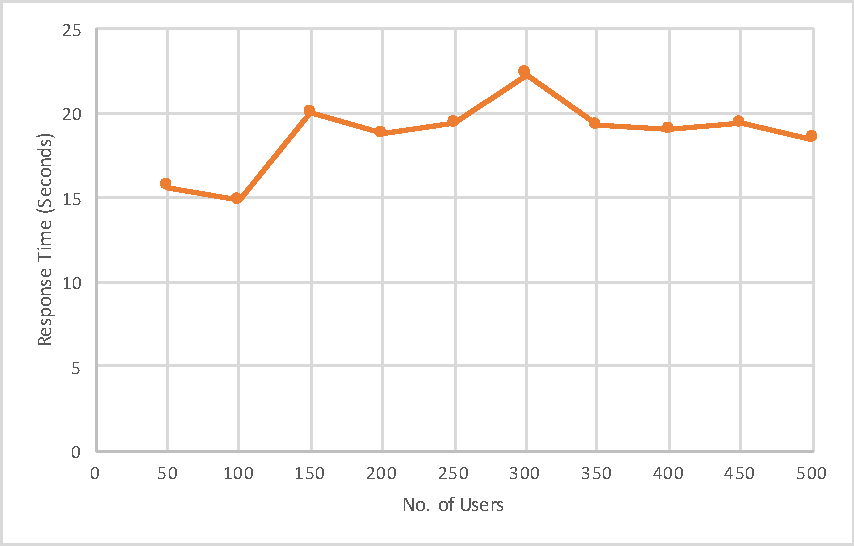
\includegraphics[width=\textwidth]{figures/siege_predictions_api_response_time_against_users.pdf}
\caption{\label{fig:siege_pre_api_response_time} Historical \& Current Timetables API Response Time (seconds) against no. of simultaneous users}
\end{figure}

\begin{figure}
\centering
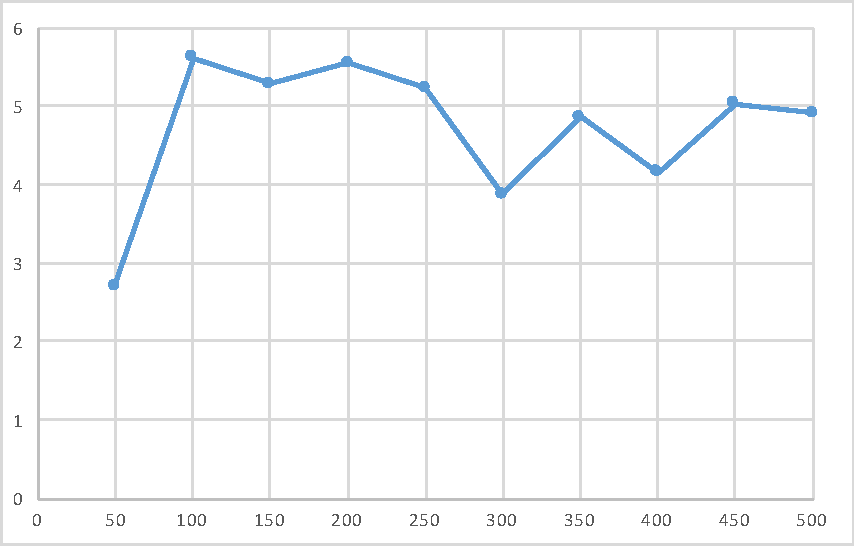
\includegraphics[width=\textwidth]{figures/siege_predictions_api_transfer_rate_against_users.pdf}
\caption{\label{fig:siege_pre_api_transfer_rate} Historical \& Current Timetables API Transaction Rate against no. of simultaneous users}
\end{figure}

\subsubsection{Reference Timetable API Performance}
\par The reference timetable API endpoint can handle about 150 users to send requests concurrently. The average response time is about 4.5 seconds. Figure \ref{fig:siege_tfl_api_availability}, \ref{fig:siege_tfl_api_response_time}, and \ref{fig:siege_tfl_api_transfer_rate} show the test results.

\begin{figure}
\centering
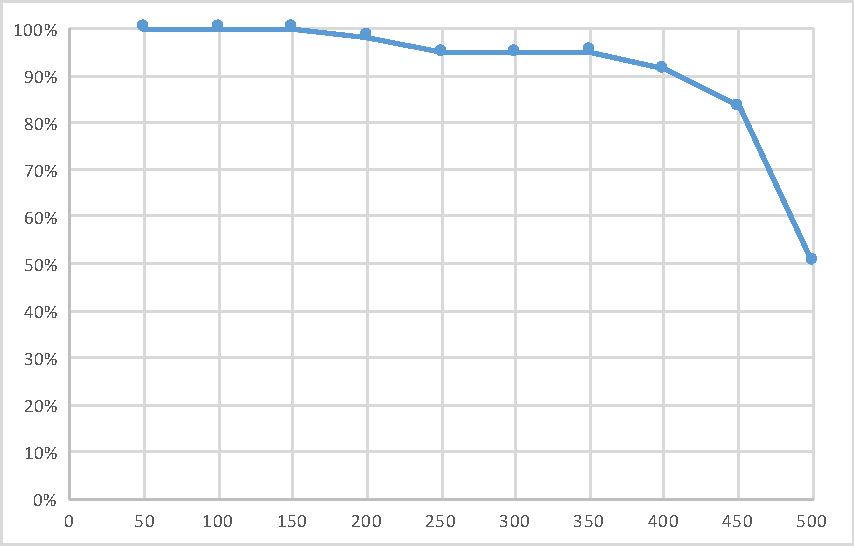
\includegraphics[width=\textwidth]{figures/siege_tfl_api_availability_against_users.pdf}
\caption{\label{fig:siege_tfl_api_availability} Reference Timetables API Availability against no. of simultaneous users}
\end{figure}

\begin{figure}
\centering
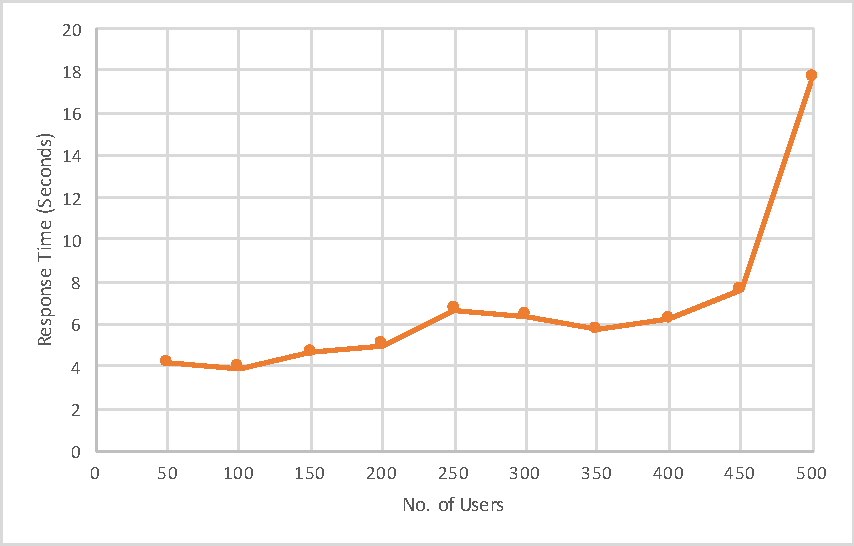
\includegraphics[width=\textwidth]{figures/siege_tfl_response_time_against_users.pdf}
\caption{\label{fig:siege_tfl_api_response_time} Reference Timetables API Response Time (seconds) against no. of simultaneous users}
\end{figure}

\begin{figure}
\centering
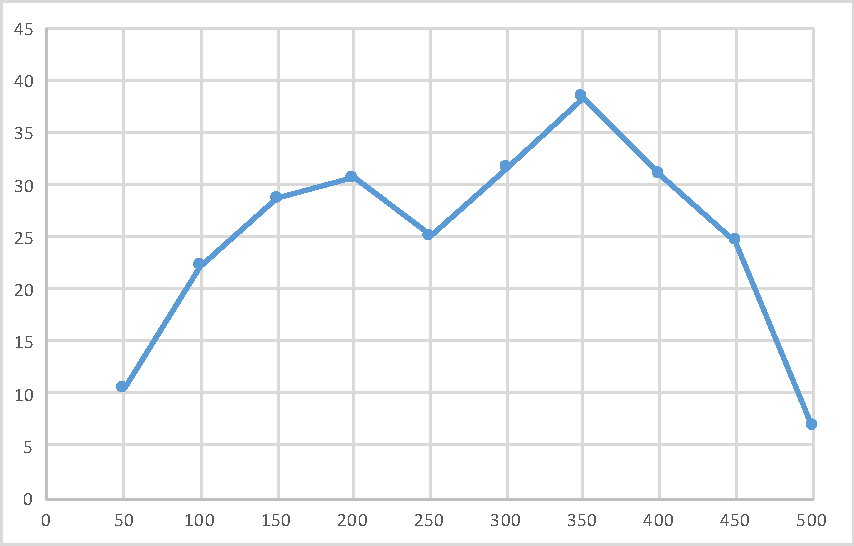
\includegraphics[width=\textwidth]{figures/siege_tfl_transfer_rate_against_users.pdf}
\caption{\label{fig:siege_tfl_api_transfer_rate} Reference Timetables API Transaction Rate against no. of simultaneous users}
\end{figure}

% \begin{figure}
% \centering
% 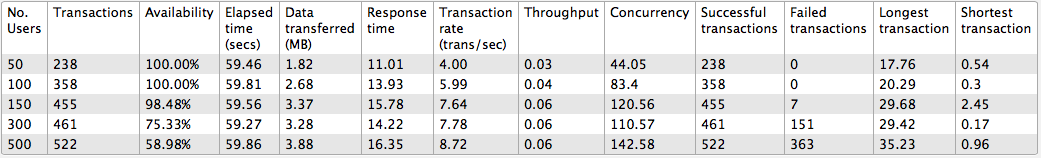
\includegraphics[width=\textwidth]{figures/performance.png}
% \caption{\label{fig:performance} Result of Performance Test with Siege}
% \end{figure}

\section{Accuracy of Predictions}
\todo[inline]{To do}
How accurate are the predictions?
\subsection{Compare predictions to real data}
We can compare the predictions generated to the live bus arrivals data stored in the arrivals table. We can calculate the standard deviation of the difference in the predicted time and actual arrival time. This value will be the direct indicator of the accuracy of the predictions.

